\section{System modeling}
\subsection{System Modeling}
Werden verwendet, um verschiedene Ansichten des Systems zu präsentieren. \newline
Es ist eine abstrakte Repräsentation und Simplifizierung des echten Systems. Details werden je nach Perspektive ausgelassen. Z.B. Kontext, Struktur Verhalten oder Interaktion.
\subsubsection{UML Diagrams} 
\begin{table}[H]
\caption{UML Diagrams}
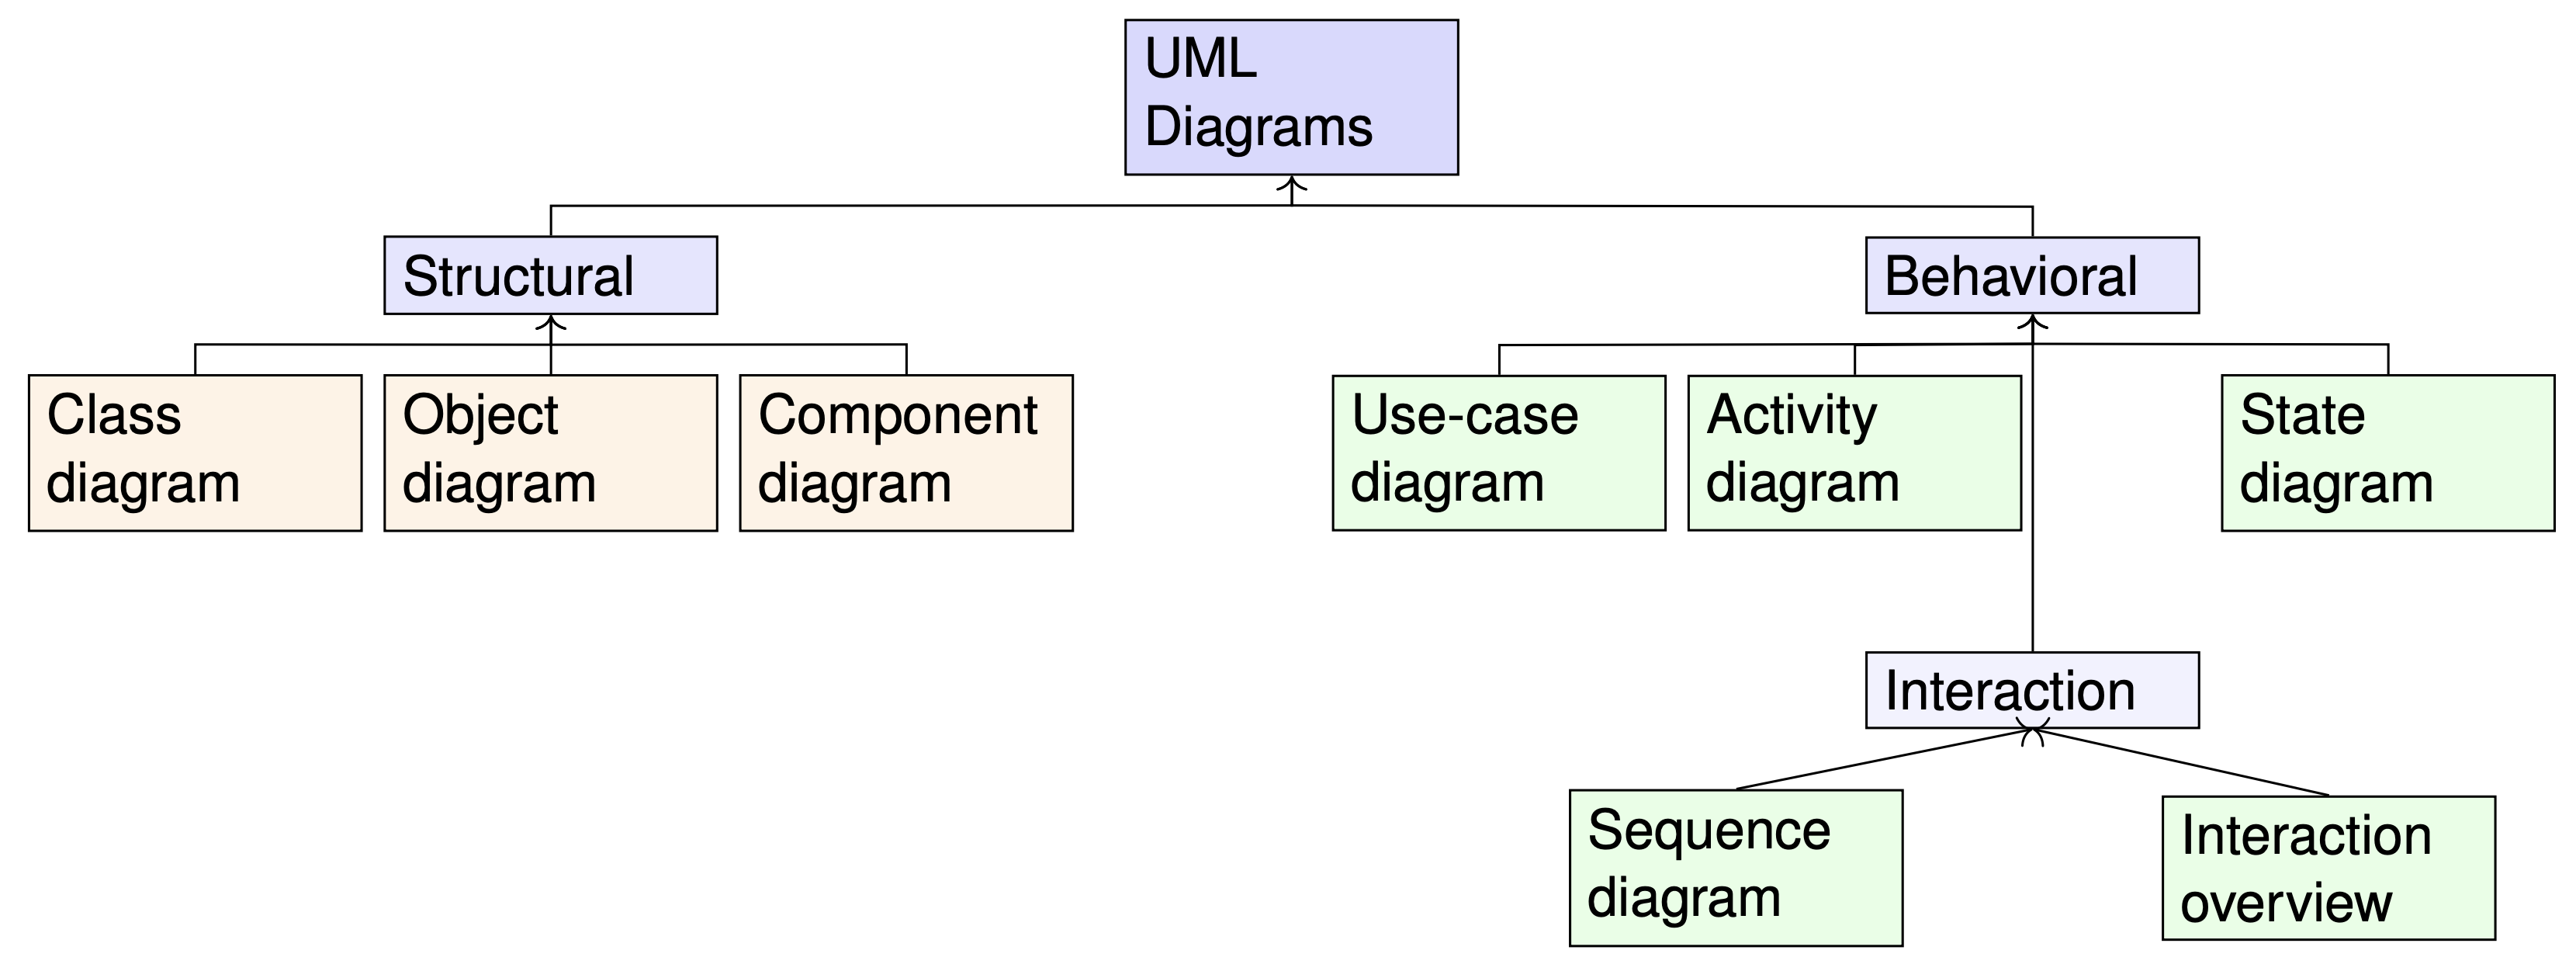
\includegraphics[scale=0.25]{UML_diagrams.png}
\end{table}
\subsection{Interaction Models}
Können für Nutzerinteraktionen, System-zu-System-Interaktionen oder Komponenteninteraktionen verwendet werden. \newline
Interaktionen können mit $\bold{Use}$ $\bold{case}$ oder $\bold{Sequenz}$ $\bold{Diagrammen}$ gemodelt werden
\begin{table}[H]
\caption{Use Case}
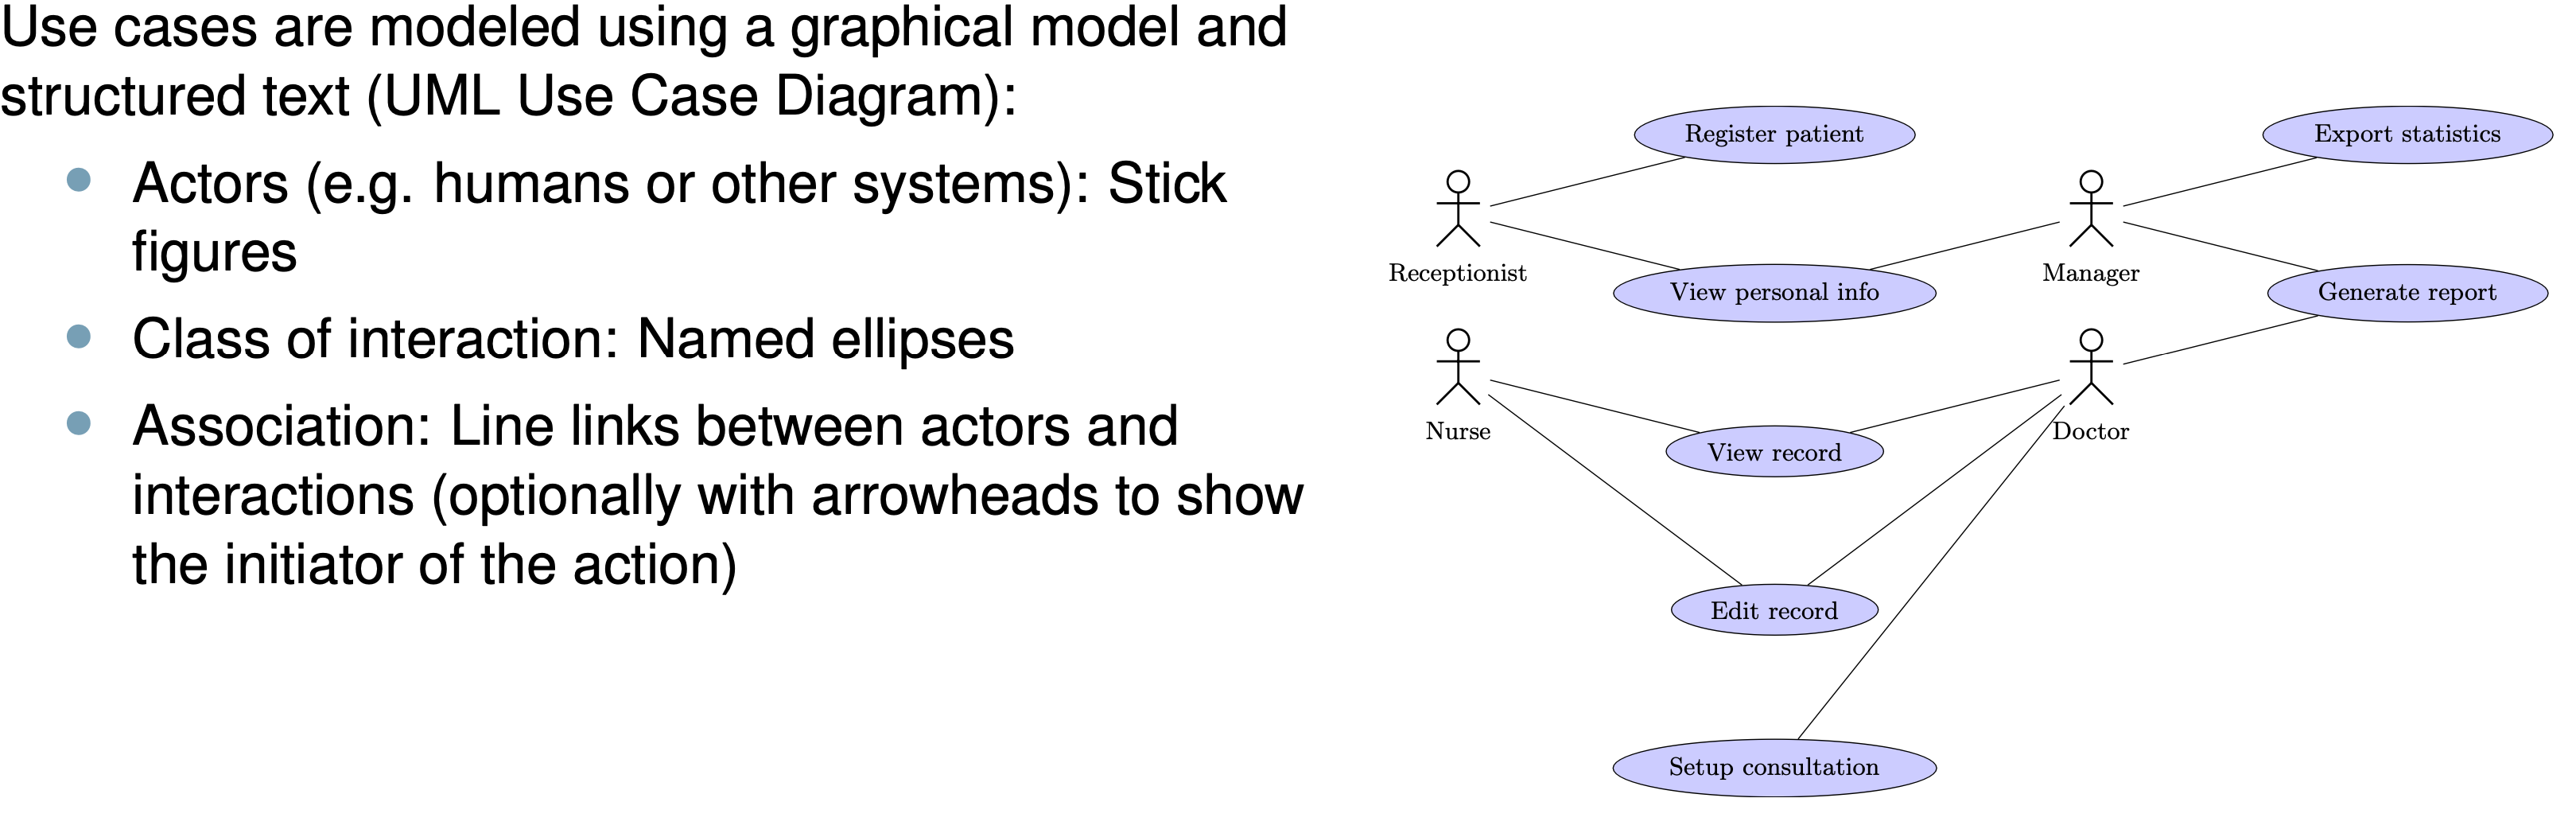
\includegraphics[scale=0.125]{Use_case_diagram.png}
\end{table}
\begin{table}[H]
\caption{Sequence}
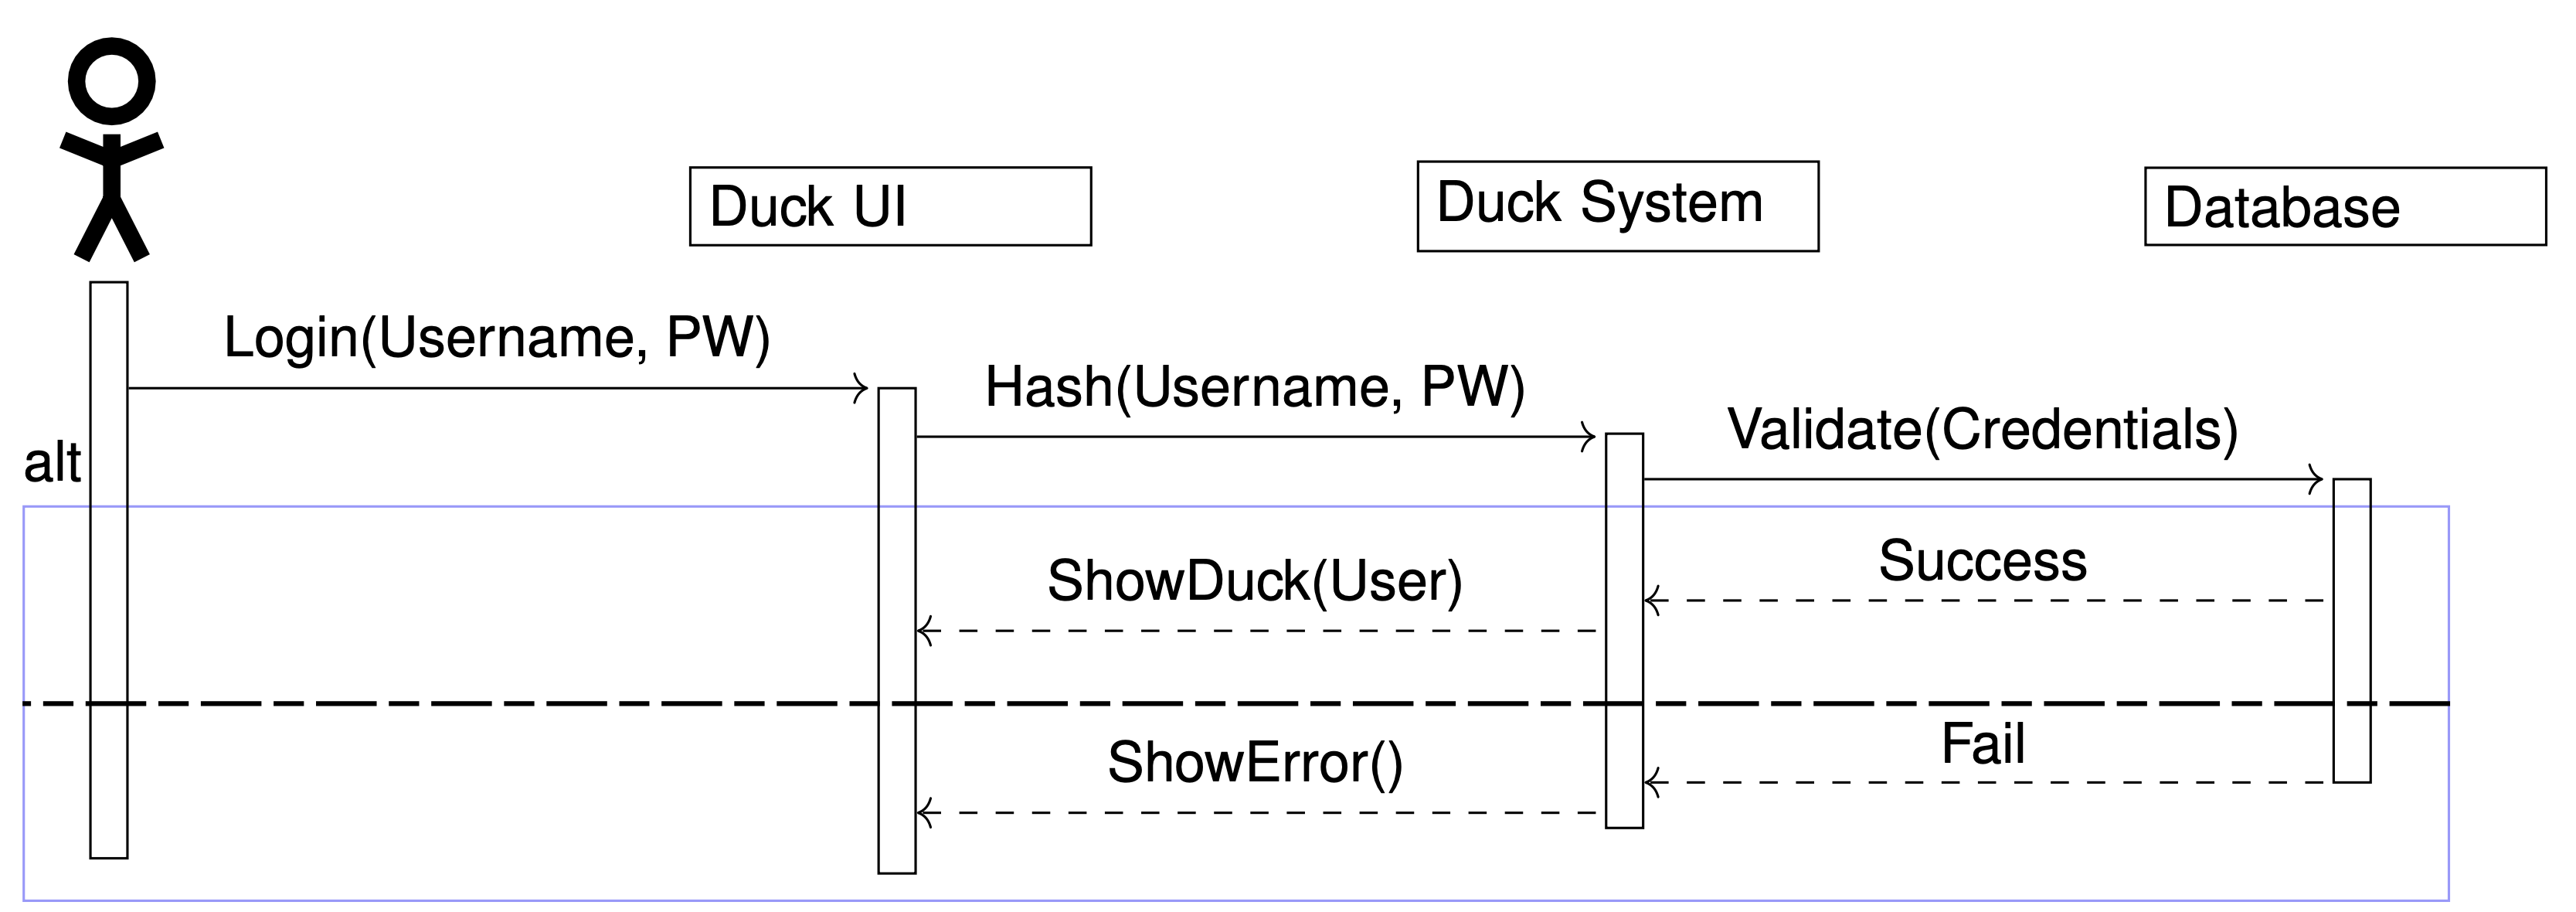
\includegraphics[scale=0.25]{Sequence_diagram.png}
\end{table}
\subsection{Structural Models}
Werden während der Designphase erzeugt und zeigen alle Komponenten und ihre Relationen
\subsubsection{Class diagrams}
$\bold{Classes}$
\begin{enumerate}
	\item Class name: Customer
	\item Atributes: +id: int 
	\item Methode name: +inquiry(): void
\end{enumerate}
$\bold{Connection}$
\begin{itemize}
	\item Association: Relation zwischen zwei Klassen (-)
	\item Directed Association: Richtung mit einem Pfeil ($\to$)
	\item Dependency: Veränderung könnte Veränderung der anderen Klasse verursachen ($- - \to$)
	\item One to One: ($1 - 1$)
	\item One to X: ($1 - 1..4$)
	\item One to many: ($1 - 1..*$)
	\item Inheritance: Nicht ausgefüllter Pfeil zu Überklasse
	\item Aggregation: (Whole $\diamond-$ Part)
	\item Composition: (Whole (Filled-)$\diamond -$ Part)
\end{itemize}
\subsection{Behavioural Models}
\subsubsection{Data-driven model}
\begin{table}[H]
\caption{Activity model}	
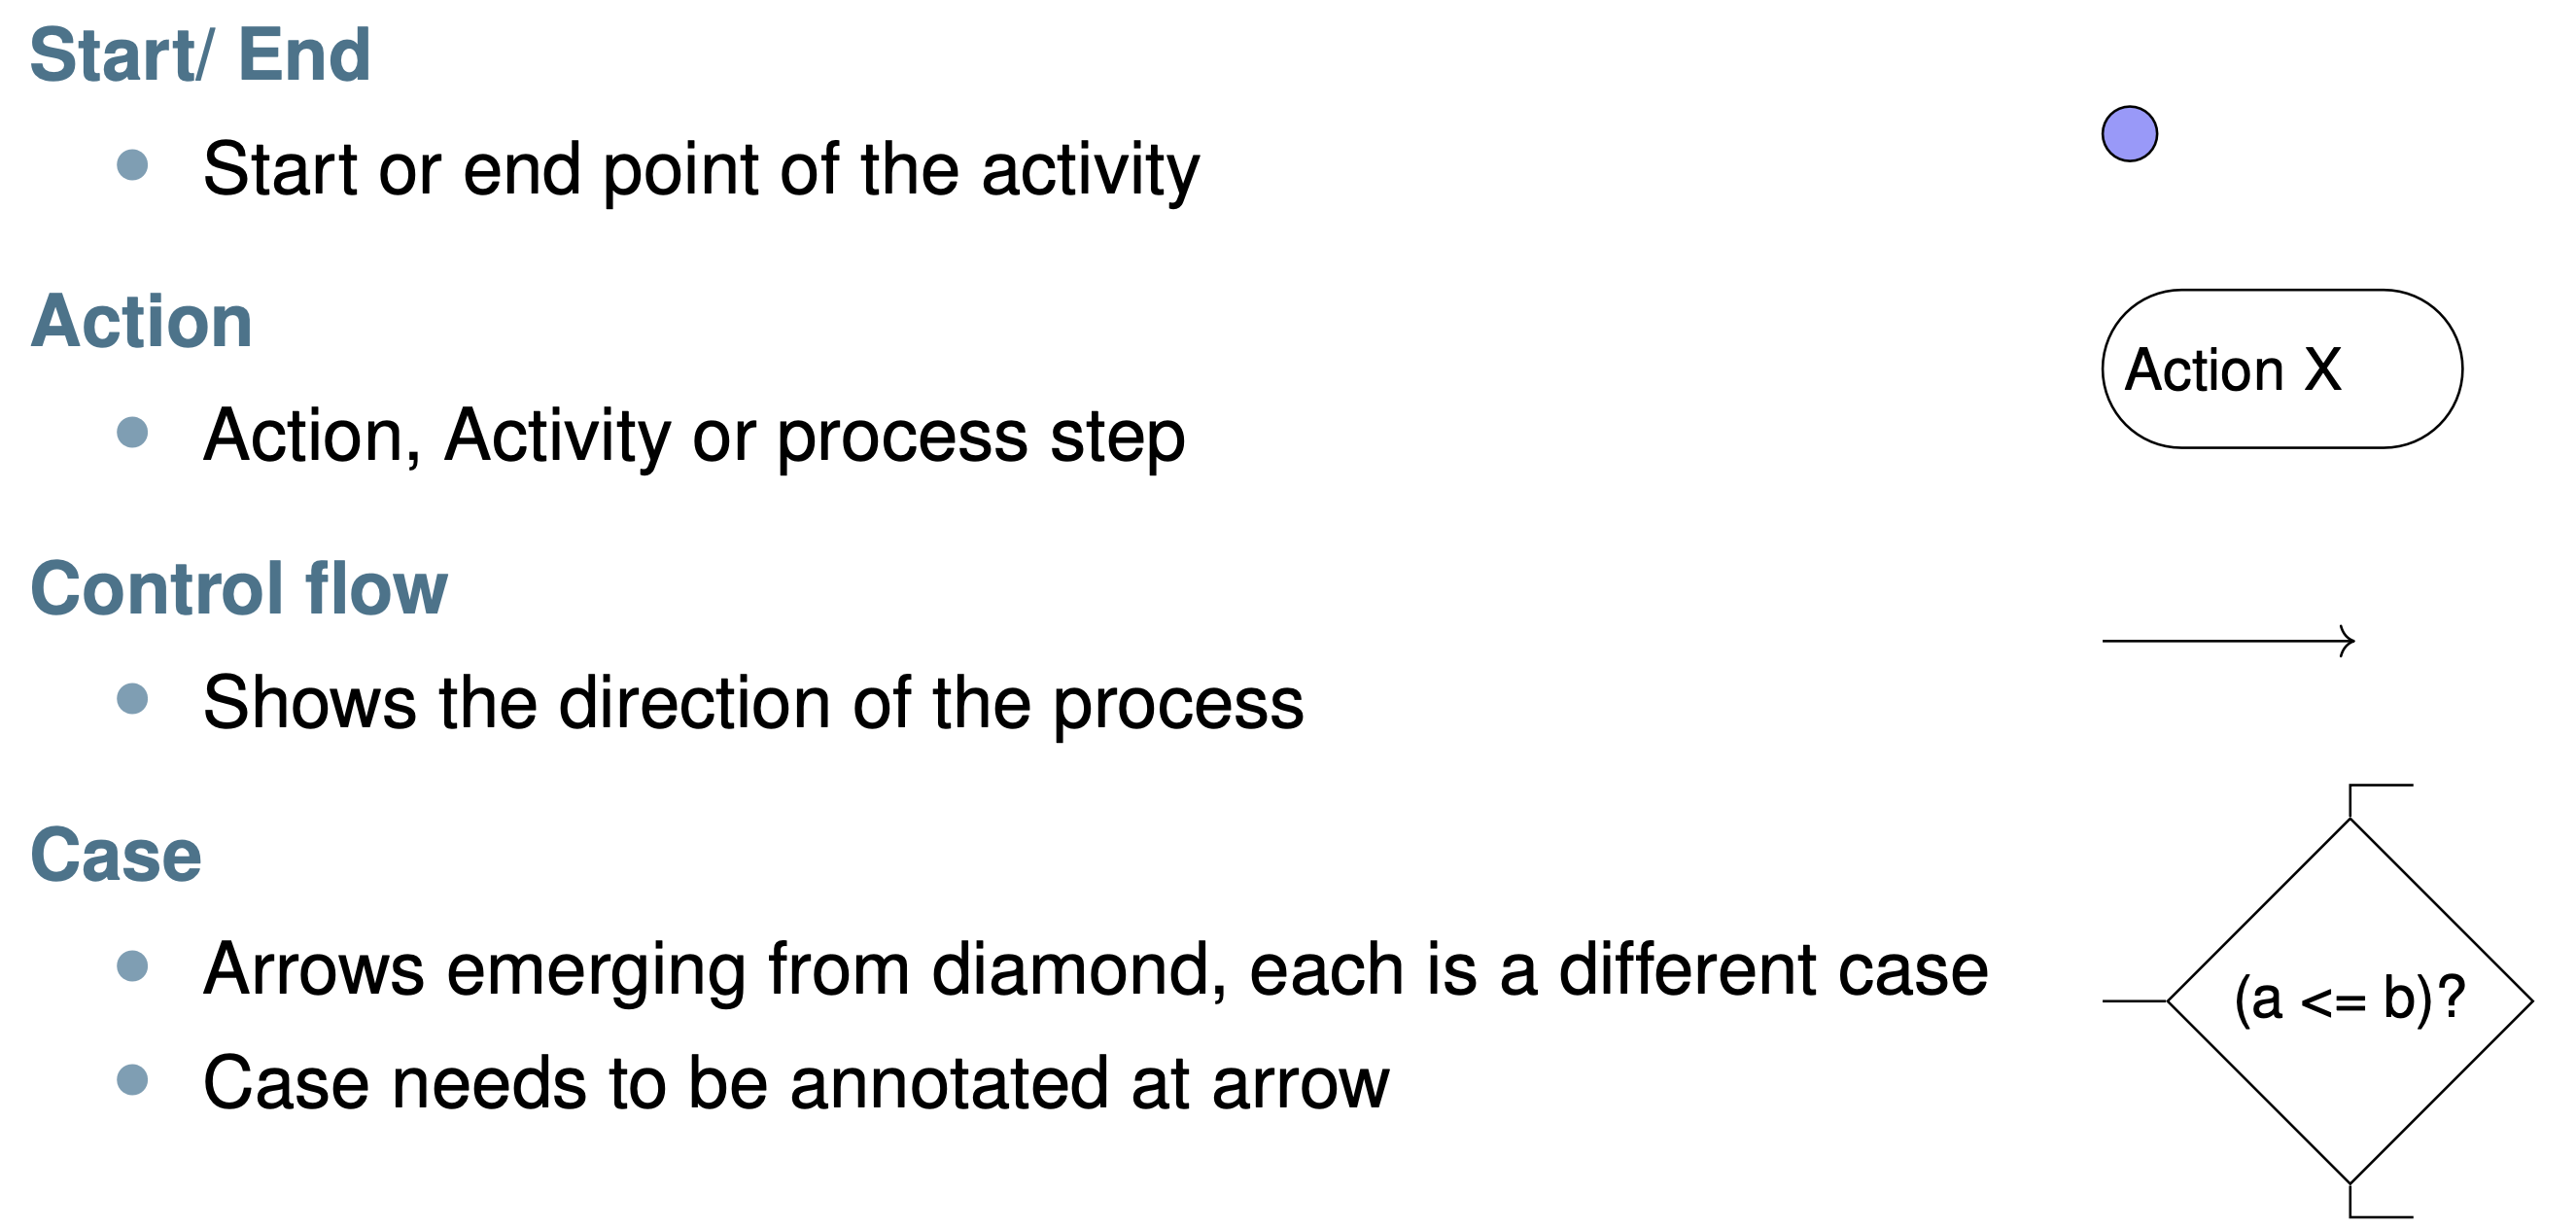
\includegraphics[scale=0.25]{Activity_model_1.png}
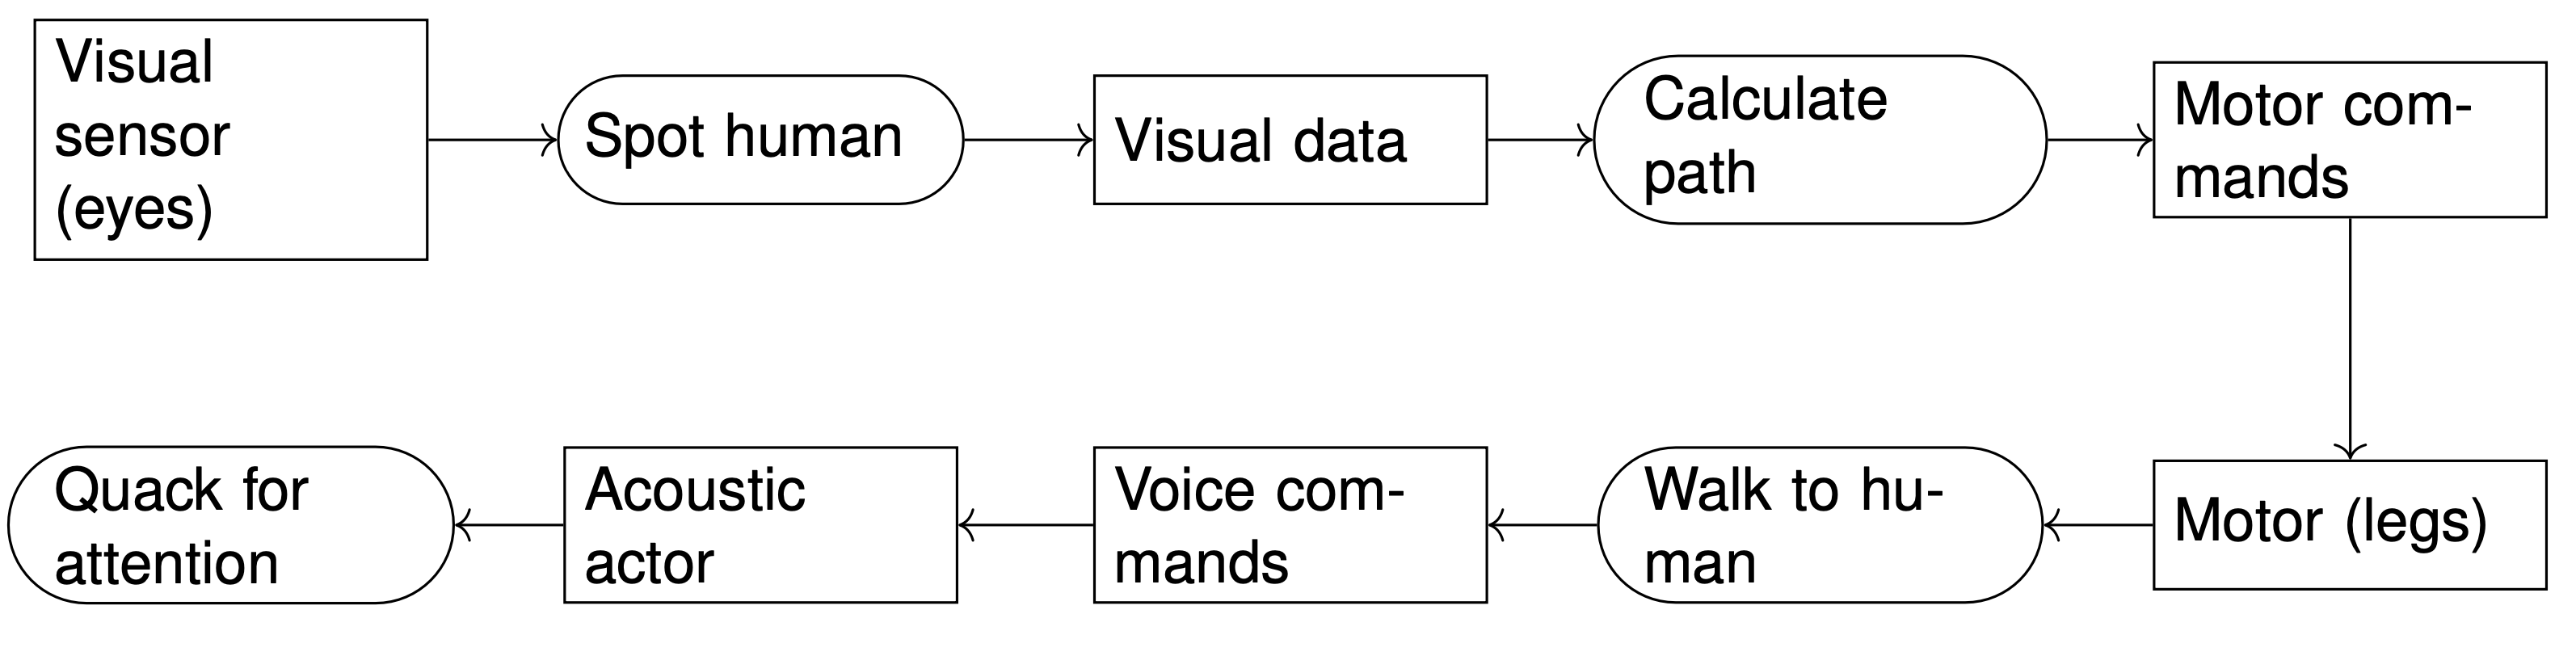
\includegraphics[scale=0.25]{Activity_model_2.png}
\end{table}
\subsubsection{Event-driven model}
\begin{table}[H]
\caption{State diagram}
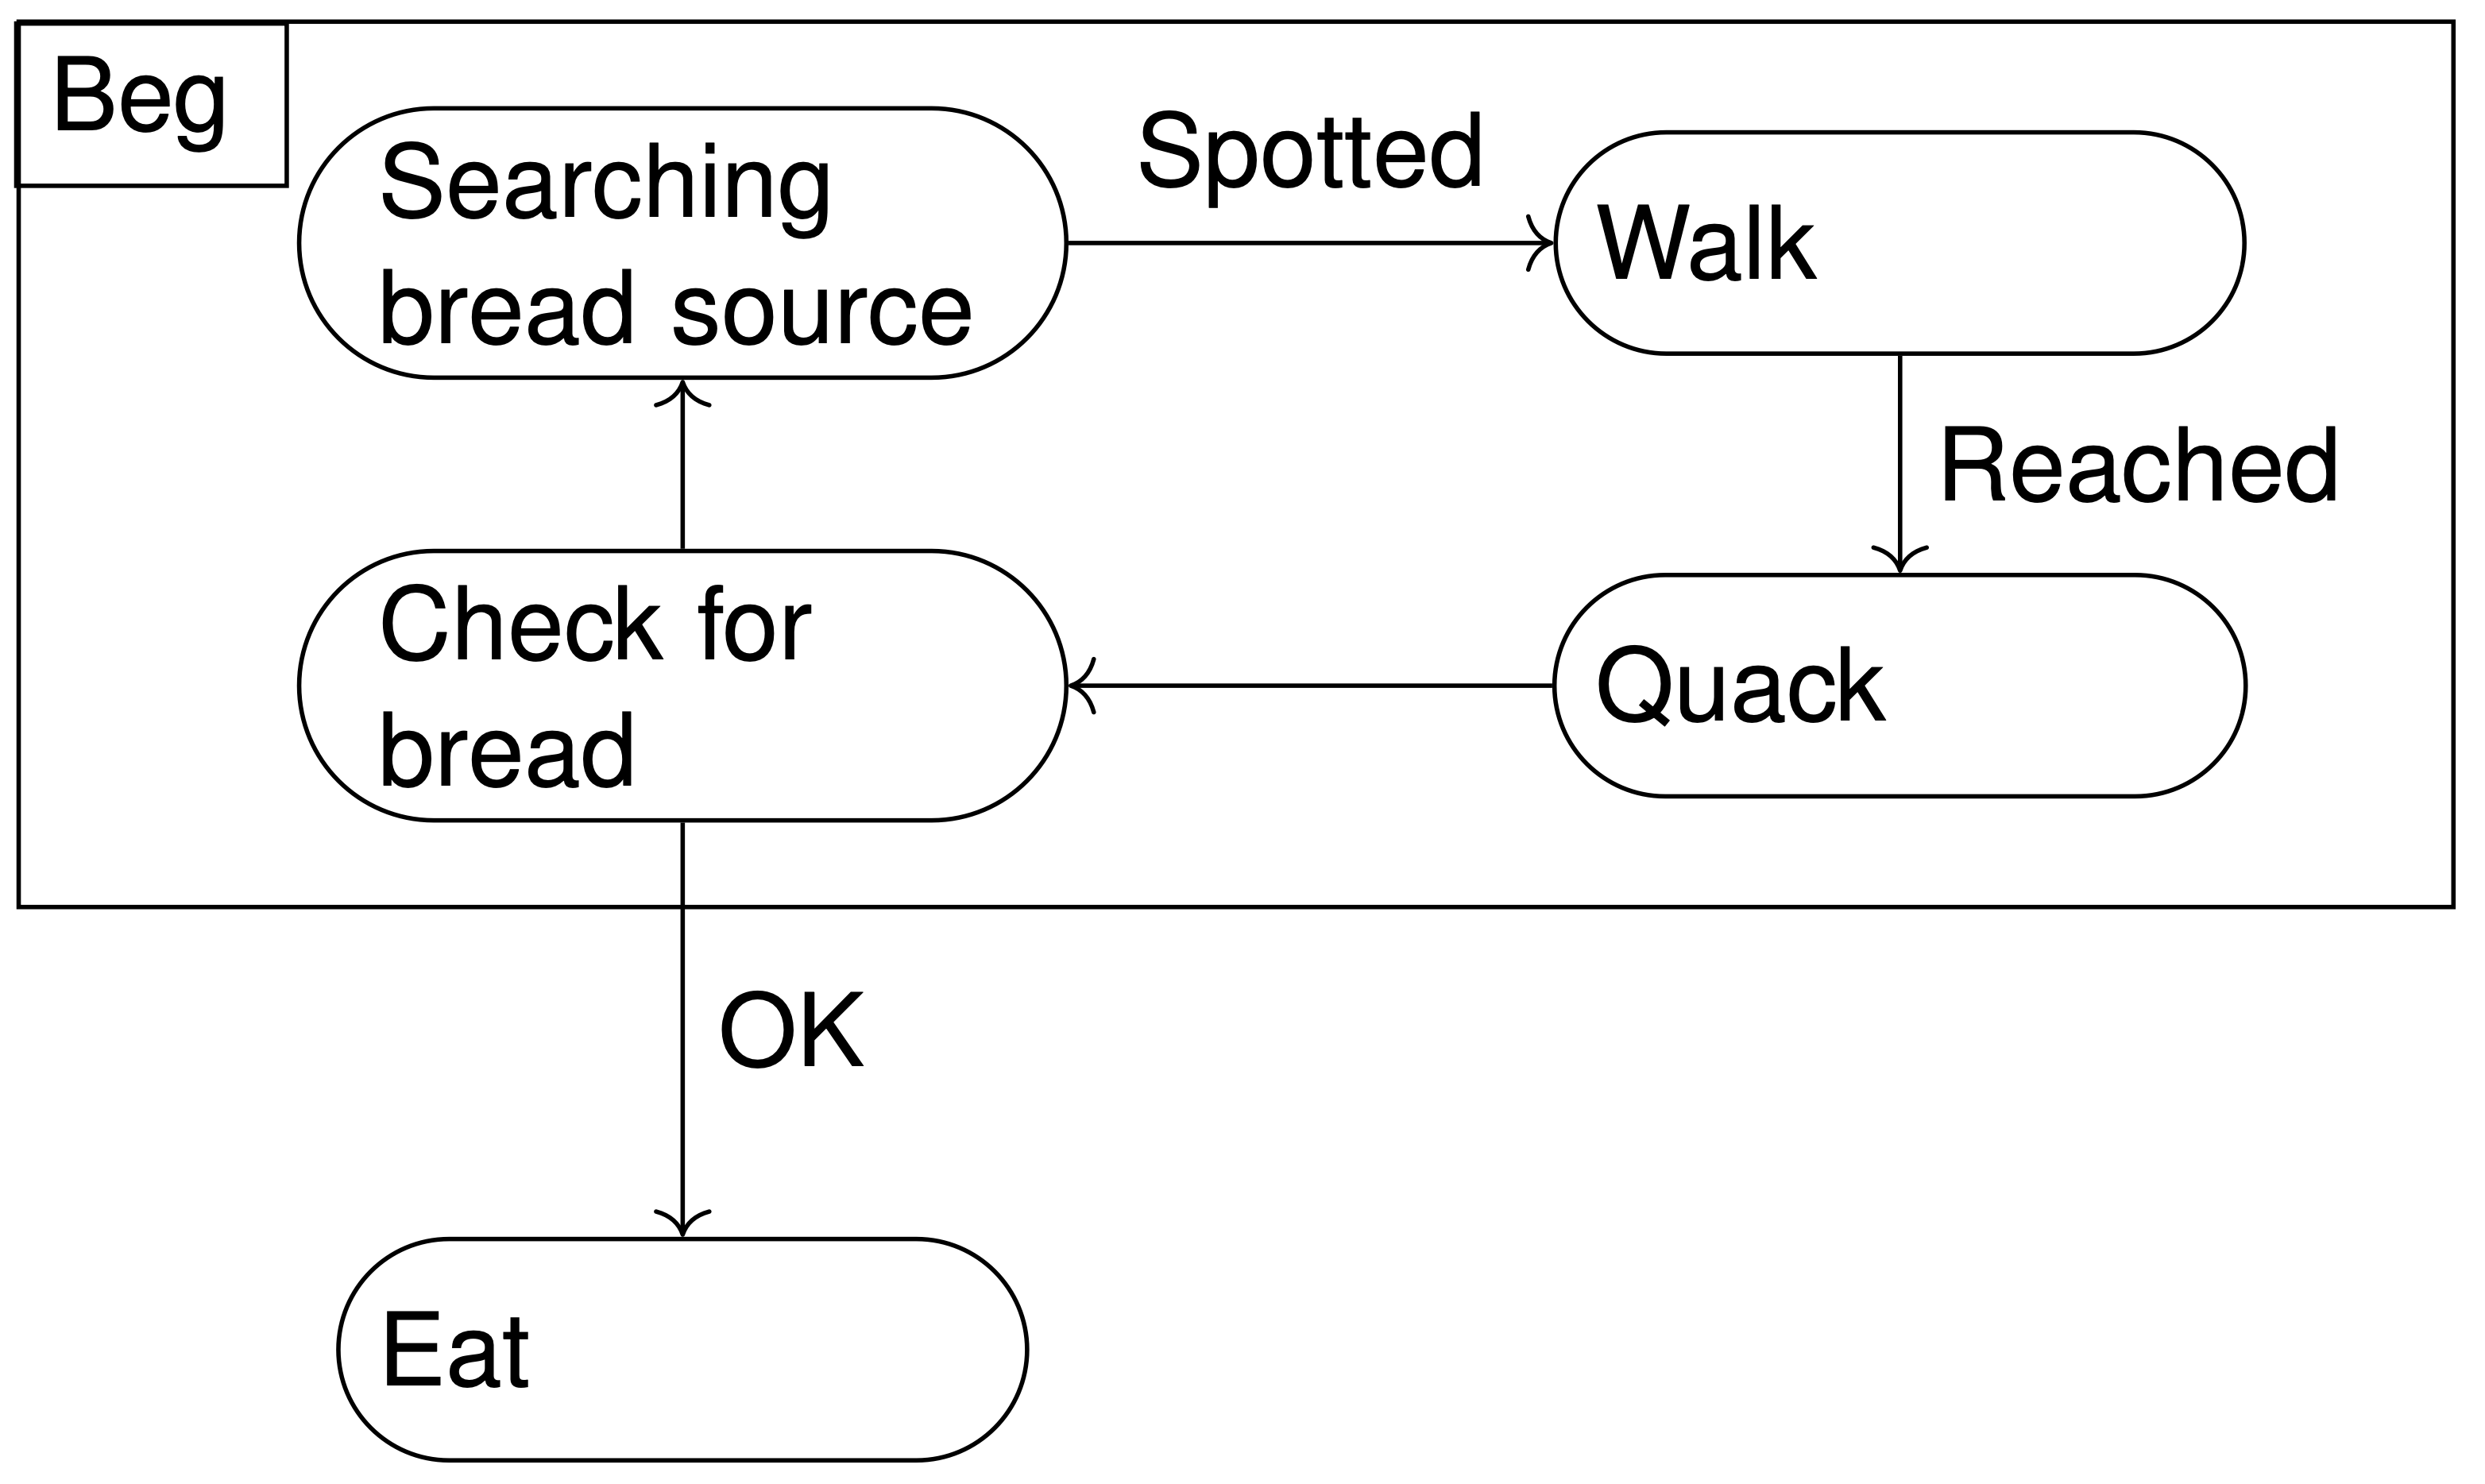
\includegraphics[scale=0.125]{State_diagram.png}	
\end{table}
\subsection{Context Models}
Kontextmodelle modellieren die Umwelt und das System, jedoch nicht die Art der Relationen, räumliche Relationen, geteilte Daten und wie das System sich verbindet.
\begin{table}[H]
\caption{Context diagram}
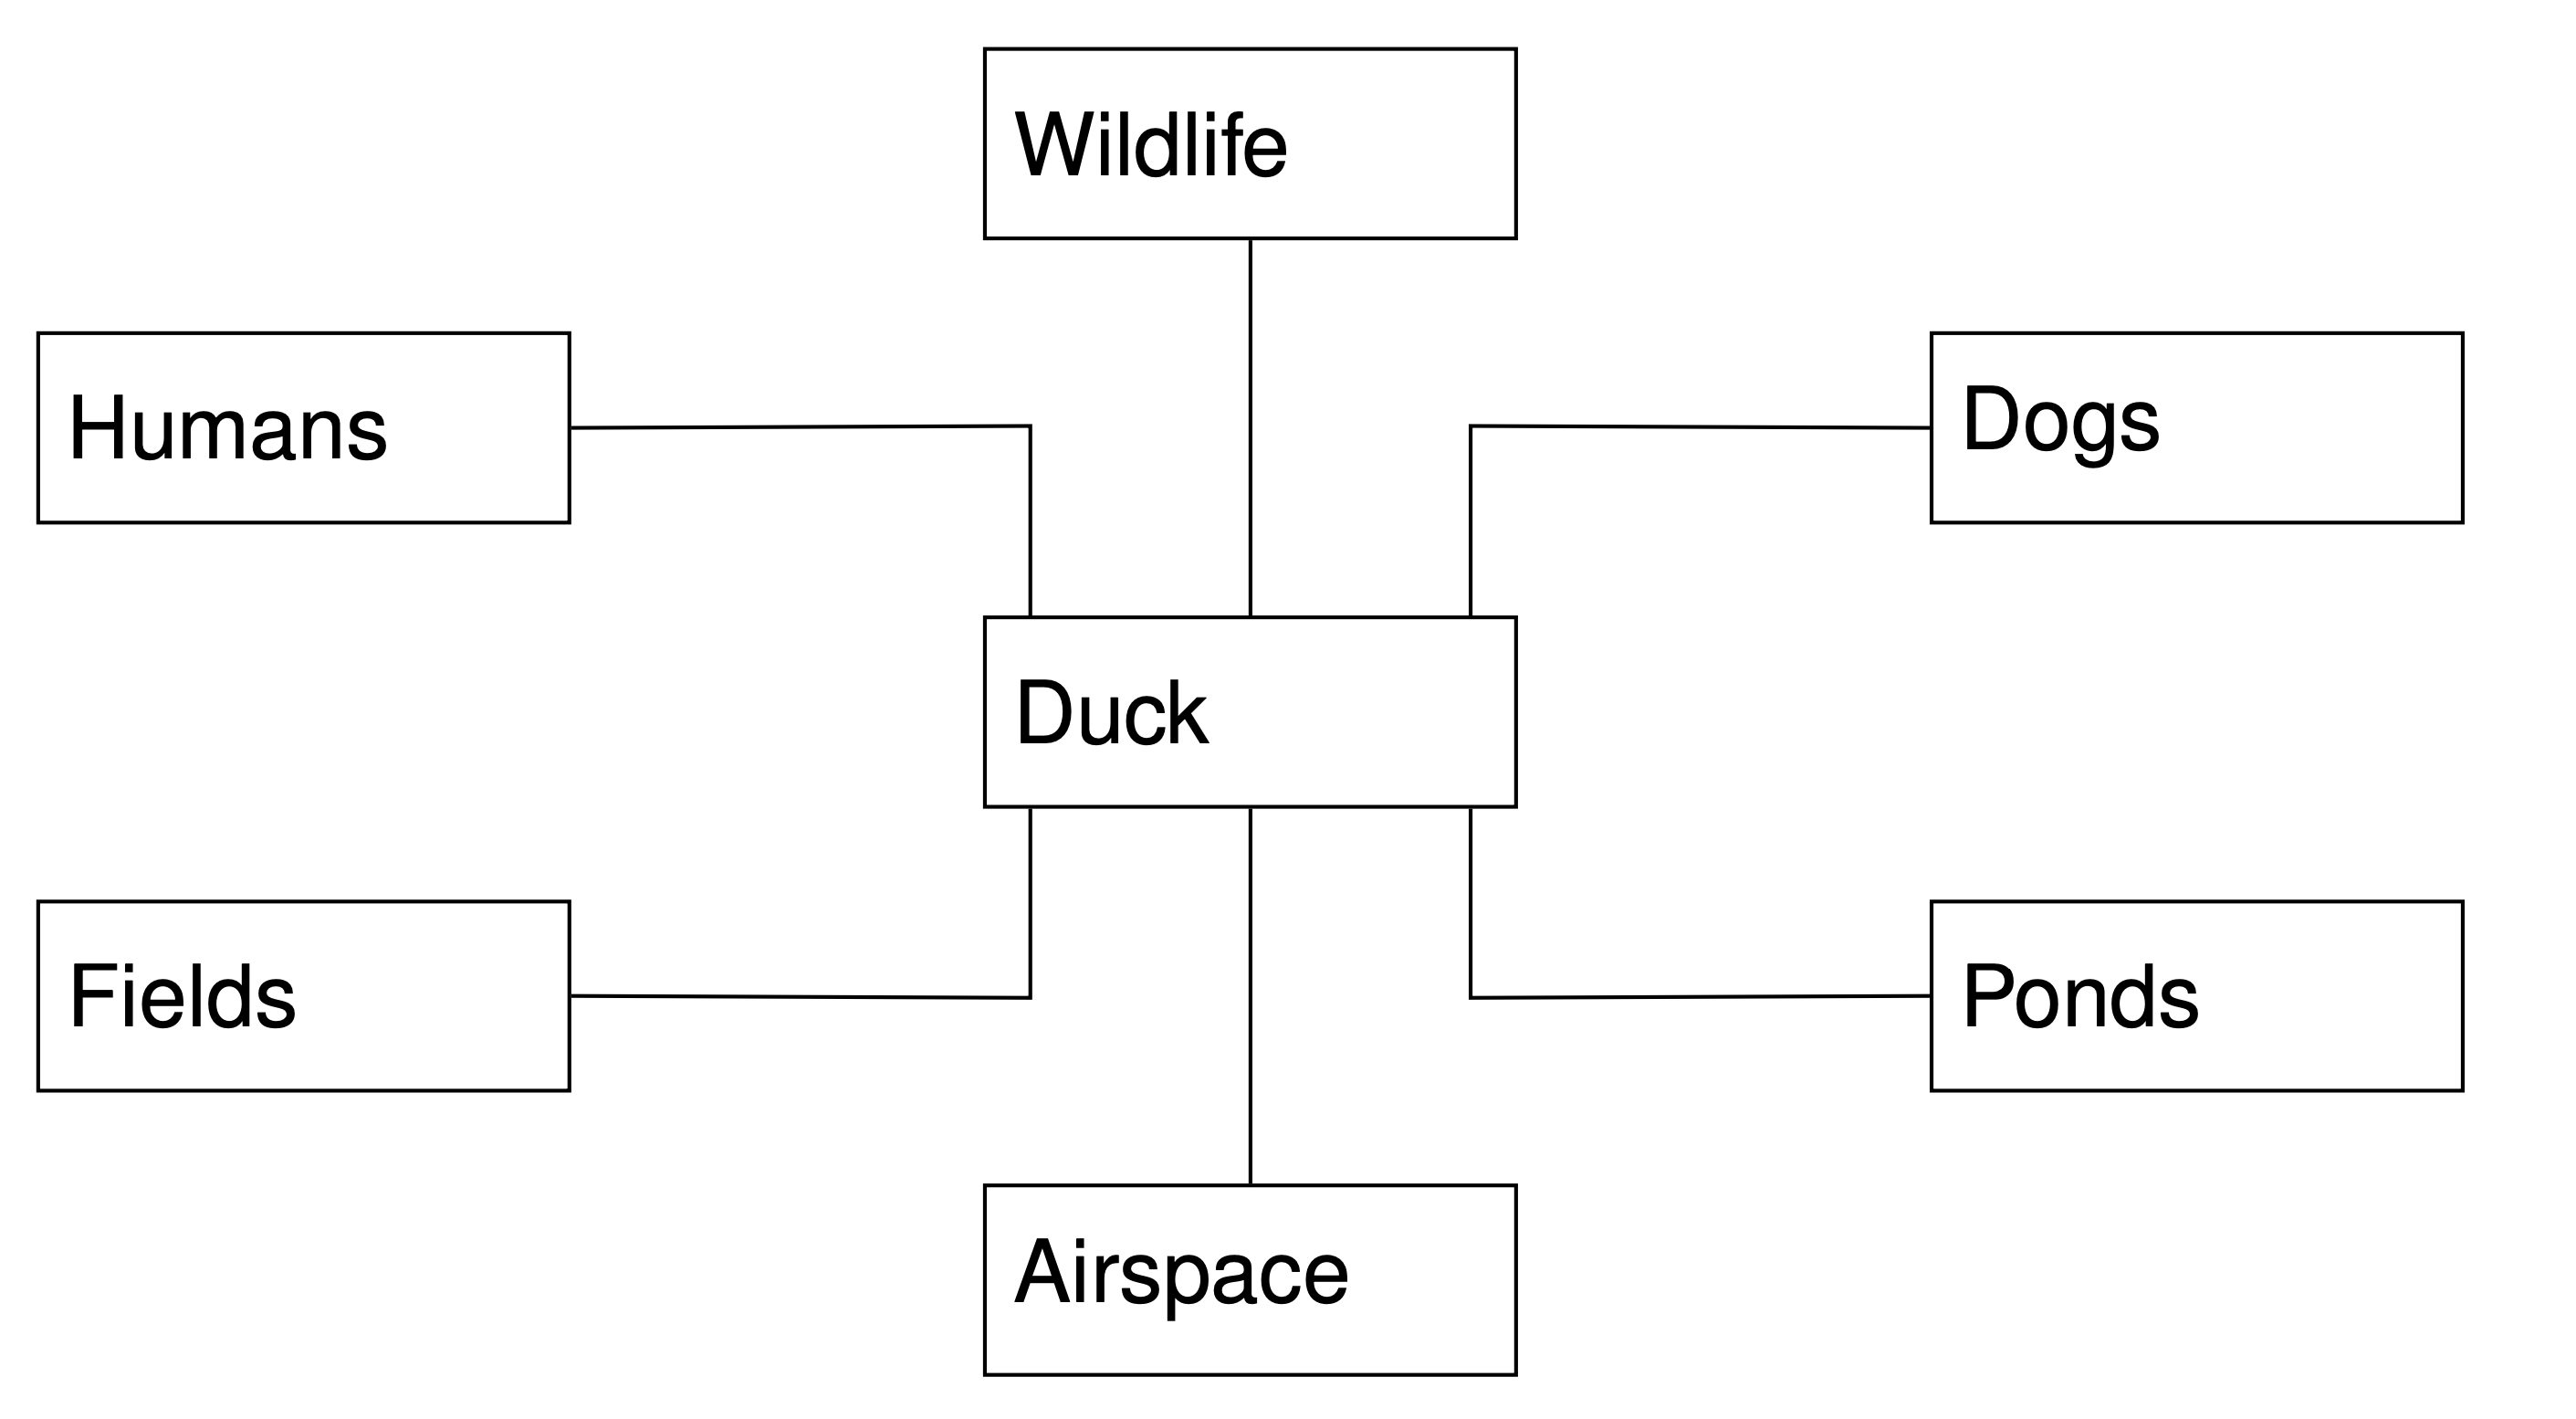
\includegraphics[scale=0.125]{Context_diagram.png}	
\end{table}
\subsubsection{Supporting models}
\begin{table}[H]
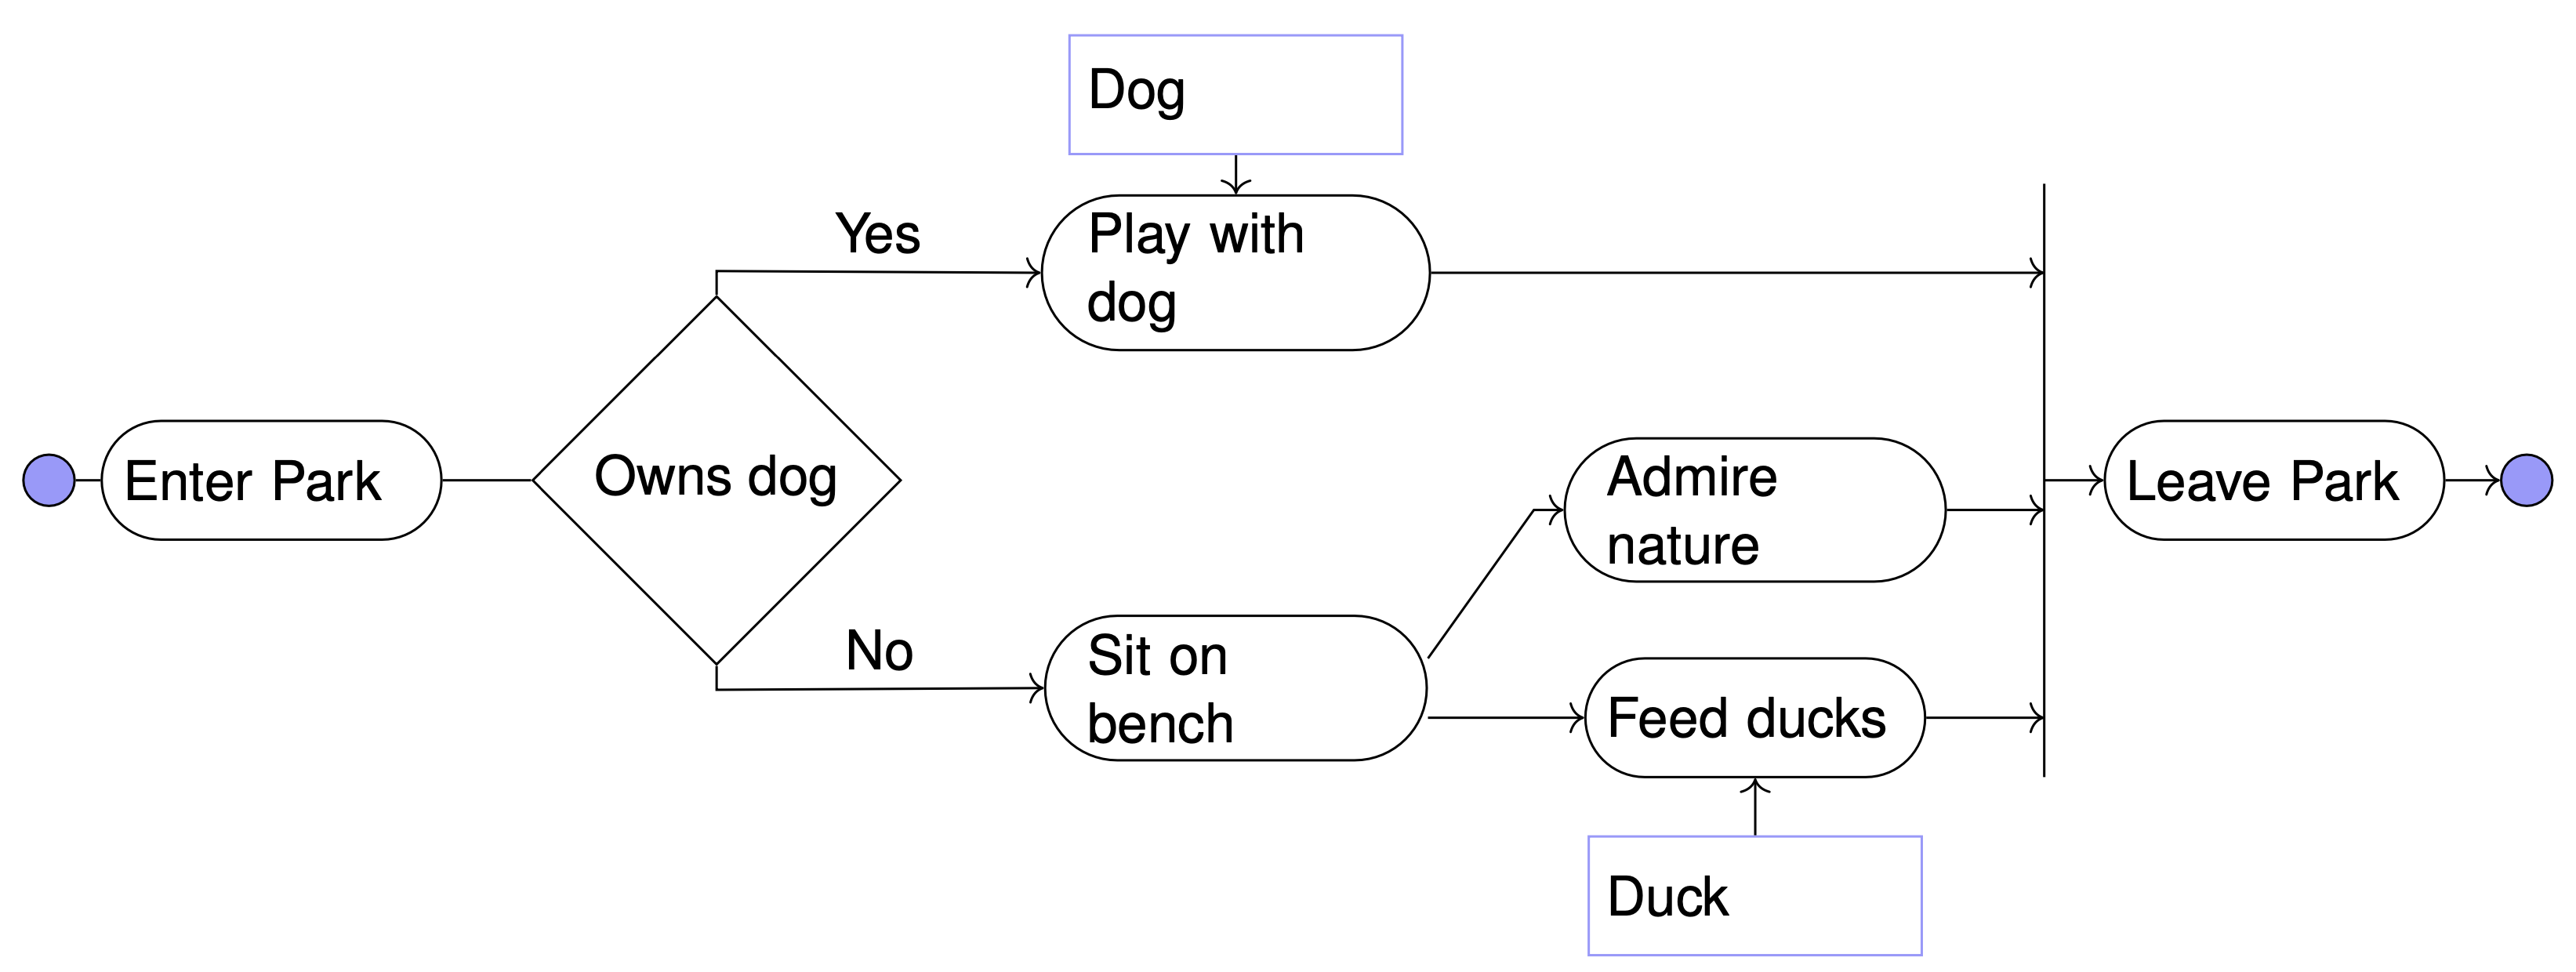
\includegraphics[scale=0.25]{Supporting_diagram.png}	
\end{table}


 




